% \begin{figure}[ht]
%     \centering
%     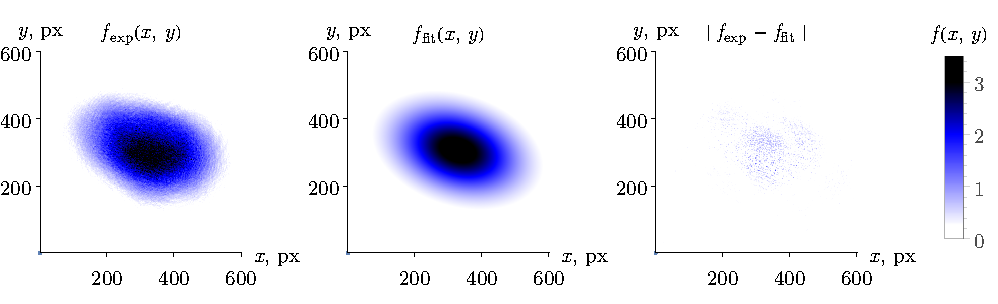
\includegraphics[width=0.6\textwidth]{../MOT/figs/fit_mot_v2.pdf}
%     \caption{Экспериментально сфотографированное распределение 
%     атомов $\sub{f}{exp}$ и аппроксимация распределения атомов $\sub{f}{fit}$
%     }
% \end{figure}

\begin{minipage}{0.68\textwidth}
Закон Бугера-Ламберта-Бера:
\begin{equation*}
    \frac{d I}{d z} = - \sigma n I,
    \hspace{10 mm} 
    \sigma = \frac{\sigma_0}{1+I/I_s + 4 (\delta/\Gamma)^2},
\end{equation*}


Распределение интенсивности:
\begin{equation*}
    \sub{f}{exp} = \ln\left(\frac{\subt{I}{D}}{I_0}\right) + \frac{\subt{I}{D} - I_0}{I_s} = \sigma_0 \int n(x, y, z) \d z.
\end{equation*}

\begin{figure}[ht]
    \centering
    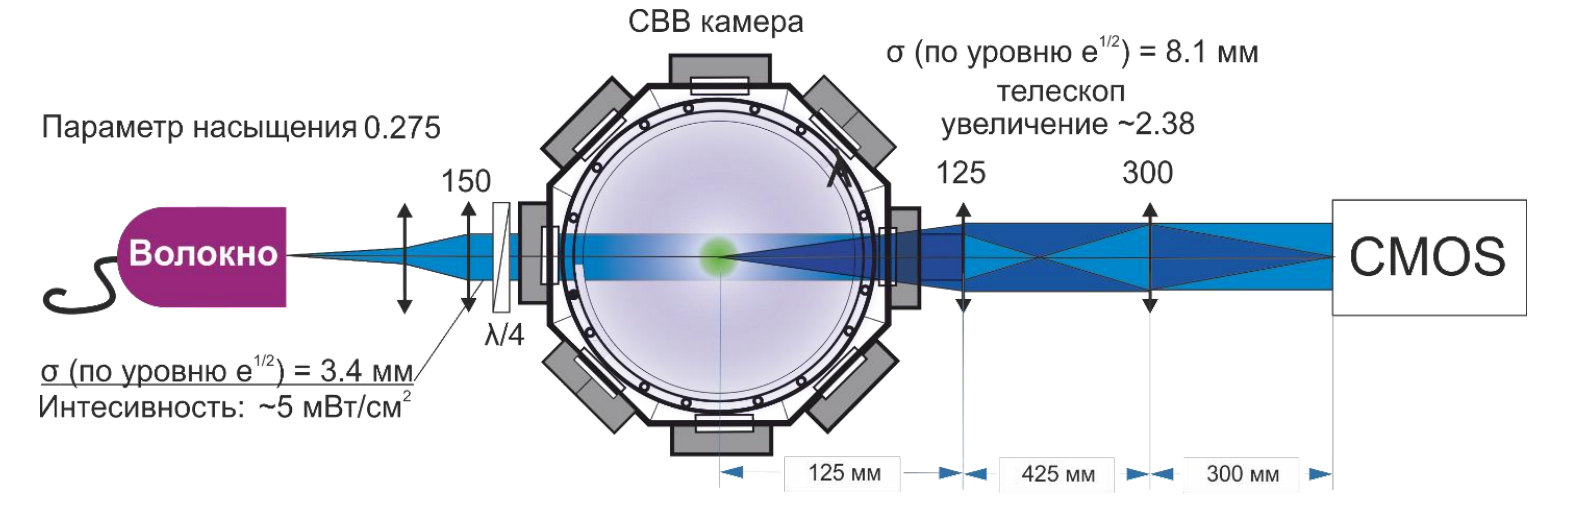
\includegraphics[width=0.9\textwidth]{../MOT/figs/detect.png}
    \caption{Схема детектирования атомов}
\end{figure}
\end{minipage}
\hfill
\begin{minipage}{0.31\textwidth}

$\subt{I}{D}$ -- фотография без атомов

$\sub{I}{0}$ -- фотография с атомами

$\sub{I}{s}$ -- интенсивность насыщения

\begin{figure}[h]
    \centering
    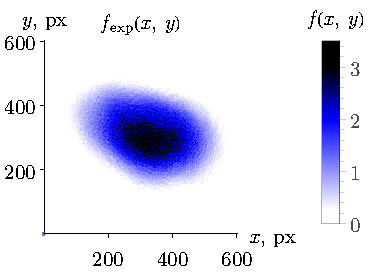
\includegraphics[width=0.99\textwidth]{../MOT/figs/fit_mot_v4.pdf}
    \caption{Фото распределения}
    %\label{fig:}
\end{figure}


\end{minipage}